%! Author = Omar Iskandarani
%! Title = Swirl String Theory (SST): A Canonical Fluid Reformulation of Relativity and Quantum Structure
%! Date = Oct, 2025
%! Affiliation = Independent Researcher, Groningen, The Netherlands
%! License = © 2025 Omar Iskandarani. All rights reserved. This manuscript is made available for academic reading and citation only. No republication, redistribution, or derivative works are permitted without explicit written permission from the author. Contact: info@omariskandarani.com
%! ORCID = 0009-0006-1686-3961
%! DOI = 10.5281/zenodo.17309679

\newcommand{\paperversion}{\textbf{v1.0.0}}
\newcommand{\papertitle}{\textbf{Swirl--String Theory: A Canonical Fluid Reformulation of Relativity and Quantum Structure}}
\newcommand{\paperdoi}{10.5281/zenodo.17309679}

%========================================================================================
% PACKAGES AND DOCUMENT CONFIGURATION
%========================================================================================
\documentclass[10pt,reprint,aps,onecolumn,nofootinbib]{revtex4-2}

\usepackage[utf8]{inputenc}
\usepackage[T1]{fontenc}
\usepackage[margin=2.3cm]{geometry}
\usepackage{amsmath,amssymb,amsfonts,bm}
\usepackage{adjustbox}
\usepackage{tikz}
\usetikzlibrary{matrix,positioning}
\usetikzlibrary{arrows.meta,positioning,calc,fit,decorations.pathmorphing}
\usetikzlibrary{matrix, positioning, fit, backgrounds}
\usepackage{siunitx}
\sisetup{per-mode=symbol,detect-weight=true,detect-family=true}
\usepackage{hyperref}
\usepackage{amsopn}
\usepackage[most]{tcolorbox}

% Canonical vector and field symbols
\newcommand{\vect}[1]{\boldsymbol{#1}} % choose \mathbf or \boldsymbol; using \boldsymbol here
\newcommand{\vv}{\vect{v}}
\newcommand{\EE}{\vect{E}}
\newcommand{\BB}{\vect{B}}
\newcommand{\HH}{\vect{H}}
\newcommand{\DD}{\vect{D}}
\newcommand{\jj}{\vect{\jmath}}

% Boxed equation helper
\newcommand{\bboxeq}[1]{\boxed{\displaystyle #1}}

% Testable-claim flag
\newcommand{\testable}{\textbf{(Testable)}}

% ===============================
% Macros (canonicalized)
% ===============================
\newcommand{\swirlarrow}{%
    \mathchoice{\mkern-2mu\scriptstyle\boldsymbol{\circlearrowleft}}%
    {\mkern-2mu\scriptscriptstyle\boldsymbol{\circlearrowleft}}%
}
\newcommand{\swirlarrowcw}{%
    \mathchoice{\mkern-2mu\scriptstyle\boldsymbol{\circlearrowright}}%
    {\mkern-2mu\scriptscriptstyle\boldsymbol{\circlearrowright}}%
}

% Canonical symbols
\newcommand{\vswirl}{\mathbf{v}_{\swirlarrow}}
\newcommand{\vswirlcw}{\mathbf{v}_{\swirlarrowcw}}
\newcommand{\SwirlClock}{S_{(t)}^{\swirlarrow}}
\newcommand{\SwirlClockcw}{S_{(t)}^{\swirlarrowcw}}
\newcommand{\Fmaxswirl}{F^{\max}_{\mkern-1mu\scriptscriptstyle\boldsymbol{\circlearrowleft}}}
\newcommand{\Fmaxswirlcw}{F^{\max}_{\mkern-1mu\scriptscriptstyle\boldsymbol{\circlearrowright}}}
\newcommand{\FmaxEM}{F^{\max}_{\mathrm{EM}}}

\newcommand{\omegas}{\boldsymbol{\omega}_{\swirlarrow}}  % swirl vorticity
\newcommand{\vscore}{v_{\swirlarrow}}                    % shorthand: |v_swirl| at r=r_c
\newcommand{\vnorm}{\lVert \vswirl \rVert}               % swirl speed magnitude
\newcommand{\rhof}{\rho_{\!f}}                           % effective fluid density
\newcommand{\rhoE}{\rho_{\!E}}                           % swirl energy density
\newcommand{\rhom}{\rho_{\!m}}                           % mass-equivalent density
\newcommand{\rc}{r_c}                                    % string core radius
\newcommand{\Lam}{\Lambda}                               % Swirl Coulomb constant
\newcommand{\Om}{\Omega_{\swirlarrow}}                   % swirl angular frequency
\makeatletter
\@ifundefined{theorem}{\newtheorem{theorem}{Theorem}}{}
\@ifundefined{corollary}{\newtheorem{corollary}{Corollary}}{}
\@ifundefined{definition}{\newtheorem{definition}{Definition}}{}
\@ifundefined{lemma}{\newtheorem{lemma}{Lemma}}{}
\makeatother

\begin{document}
\title{\papertitle}
\author{Omar Iskandarani}
\affiliation{Independent Researcher, Groningen, The Netherlands}
\thanks{ORCID: 0009-0006-1686-3961, \\ DOI: \paperdoi}
\date{\today}

%==================== ABSTRACT (revised) ====================
\begin{abstract}
We present \emph{Swirl--String Theory} (SST), a fluid–topological framework in which matter and radiation are modeled as quantized vortex loops (“swirl strings”) in an incompressible, non-dissipative condensate. Within SST, classical gravitational phenomenology \emph{emerges} as a collective pressure effect in flat space, while local swirl flows \emph{recover} relativistic time-dilation kinematics. We formulate a covariant effective field theory on a preferred foliation, show how topological quantization organizes a discrete particle spectrum, and outline a route by which gauge structures may be \emph{derived} from orientational textures of the medium. A modified Faraday law is proposed in which time-varying swirl areal density sources an electromotive impulse; this yields geometry-independent, quantized flux signatures that serve as explicit falsification targets. Wave–particle duality is described via R/T phase dynamics (unknotted vs.\ knotted states), with measurement modeled as an R$\leftrightarrow$T transition. We compare SST with Kelvin’s vortex lineage, analogue-gravity programs, and emergent-gauge constructions, emphasizing where SST \emph{recovers} established limits (Newtonian gravity, Maxwell electrodynamics, quantum interference) and where it \emph{predicts} deviations that are testable in BECs, superconducting films, and attosecond spectroscopy. All equations use SI units with dimensional checks. Our aim is a parameter-light, topological account that complements standard formulations and invites direct experimental appraisal.
\emph{Keywords:} vortex dynamics; topological fluid; emergent gauge theory; time dilation; quantum measurement; attosecond spectroscopy
\end{abstract}
\maketitle

%==================== INTRODUCTION ====================
\section{Introduction}\label{sec:intro}
    Reconciling General Relativity (GR) with Quantum Mechanics (QM) remains difficult because GR treats spacetime as dynamical and curved, whereas quantum field theories (QFT) typically operate on a fixed background. Swirl–String Theory (SST) approaches this tension by positing a unified substrate: a flat-space, incompressible condensate that supports and constrains all excitations.~\footnote{Several preprints by the author are cited to reflect distinct developments of the SST framework. Each addresses separate derivational or phenomenological components. Peer-reviewed validation is ongoing.}

    \subsection*{Motivation: Recasting the GR–QM Mismatch}
        The long–standing mismatch between the Standard Model (SM) and GR suggests re-examining some starting assumptions. SST recasts curvature as effective fluid kinematics within a background Euclidean manifold. In this picture, what is interpreted as gravity \emph{emerges} from pressure and flow gradients in the condensate rather than from a fundamental geometric interaction. Treating both gravitational and quantum effects within one hydrodynamic framework \emph{aims} to clarify shared mechanisms while preserving empirical constraints from GR and the SM.

    \subsection*{Historical Lineage: From Vortex Atoms to Analogue Gravity}
        SST fits within a broader tradition that links topological fluid structures to matter. Early ideas—such as Kelvin’s vortex atoms—anticipated the use of knotted, conserved circulations as building blocks. Modern developments in knot theory, quantized circulation, and analogue gravity deepen this thread: horizons and other curved–spacetime analogues can be \emph{recovered} in superfluids and Bose–Einstein condensates. SST draws on this lineage by using the stability of vortex dynamics to \emph{derive} a durable particle spectrum.

    \subsection*{SST Proposition: A Topological Fluid Substrate for Particles and Interactions}
        SST posits a single universal medium—the “swirl” condensate—characterized by effective density, core swirl speed, and core radius. Physical observables such as mass, forces, and time dilation \emph{emerge} from topologically protected excitations: knotted swirl strings. Formally, the framework resembles a modern Lorentz–Ether–style construction: it lives on a flat 4D manifold with an absolute time parameter and a preferred foliation set by the condensate’s unit timelike flow. The appeal of this background lies in what it may \emph{predict}: topological constraints on mass generation and the \emph{recovery} of SM–like gauge structure offer a path toward fewer free parameters than many effective models. At the same time, SST accepts empirical equivalences with standard formulations wherever they obtain and treats departures as testable claims rather than assumptions.

    \subsection*{Relation to Emergent-Gravity Programs}
        Conceptually, SST aligns with approaches in which gravity \emph{derives} from statistical or informational tendencies rather than standing as a separate fundamental interaction. In SST, a time–varying swirl density acts like an entropy– or information–density field. Resulting hydrodynamic gradients track the gradient of this swirl–based entropy and \emph{recover} attractive behavior consistent with gravitational phenomenology. This analogy is used as an organizing principle rather than as a claim of superiority; points of agreement and potential deviation are presented as targets for calculation and experiment. While string theory often pursues unification through extra–dimensional vibrational modes~\cite{Susskind2003}, SST frames unification in terms of topological fluid structures in a fixed 4D background. Consistent with calls for sharper empirical criteria~\cite{Hossenfelder2018}, we emphasize falsifiable consequences (Secs.~\ref{sec:em}, \ref{sec:falsifiability}).


%==================== CORE POSTULATES ====================
\section{Core Postulates of Swirl–String Theory}\label{sec:postulates}
    SST is defined by six axioms that constrain the dynamics and properties of a universal condensate and its topological excitations. Core postulates follow from SST Canon v0.5.10~\cite{sstCanon}, with corresponding derivations in~\cite{sstLagrangian}.

    \subsection*{Axioms from the Canon v0.5.10}
        \begin{enumerate}
        \item \textbf{Incompressible swirl condensate.} Physics is modeled on Euclidean $\mathbb{R}^3$ with an absolute time $t$. The background substrate is a frictionless, incompressible fluid ($\nabla \cdot \vv=0$) that supplies the kinematic stage on which all excitations evolve.

        \item \textbf{Swirl strings as knotted topological excitations.} Particles and field quanta are represented by closed, stable vortex filaments (``swirl strings''). Their discrete quantum numbers \emph{derive} from knot topology and linking invariants, providing a topological state space for matter and radiation.

        \item \textbf{Quantized circulation ($\Gamma=n\kappa$).} The circulation of the swirl velocity $\vect{v}_{\mkern-2mu\scriptscriptstyle\boldsymbol{\circlearrowleft}}$ around any closed loop $C$ is \emph{quantized} in integer multiples of a fundamental quantum $\kappa$,
        \[
            \Gamma = n\kappa,
        \]
        with $\kappa=h/m_{\mathrm{eff}}$ linking topological class to a quantum scale, in parallel with Onsager–Feynman quantization in superfluids~ \cite{Onsager1949}.

        \item \textbf{Swirl clocks and local time dilation ($S_t$).} Local proper time is set kinematically by the local tangential swirl speed $v$, with
        \begin{equation}
        S_t \;=\; \frac{dt_\text{local}}{dt_\infty} \;=\; \sqrt{1-\frac{v^2}{c^2}},
        \label{eq:swirlclock}
        \end{equation}
        which \emph{recovers} the standard special–relativistic time-dilation factor. In the SST picture, high swirl speeds co-vary with deeper effective gravitational potentials, so clocks slow where the medium’s flow is strongest. The claim is kinematic equivalence, not empirical replacement: SST aims to match established relativistic tests while offering a medium-based account of the same effects.

        \item \textbf{Dual R-phase and T-phase states.} Swirl strings exhibit a two-phase description: an extended, unknotted R-phase (radiative, wave-like, effectively massless) and a localized, knotted T-phase (tangible, particle-like, mass-carrying). Quantum duality is modeled as a dynamical R$\leftrightarrow$T transition.

        \item \textbf{Canonical knot–particle correspondence (illustrative mapping).} Specific knot classes are proposed to \emph{correspond} to particle species. A representative assignment places charged leptons on torus knots (e.g., electron $\leftrightarrow$ trefoil $3_1$) and quarks on chiral hyperbolic knots (e.g., up quark $\leftrightarrow 5_2$, down quark $\leftrightarrow 6_1$). Massless bosons (e.g., photons) are modeled as unknotted R-phase torsional excitations. These mappings are presented as testable, calculable hypotheses anchored in topological invariants rather than as presupposed identities.
        \end{enumerate}

%==================== LAGRANGIAN ====================
\section{Lagrangian and Field-Theoretic Framework}\label{sec:lagrangian}
    The dynamical content of SST is organized as a covariant effective field theory (EFT) defined on a preferred time foliation supplied by the condensate flow~ \cite{sstLagrangian}. The formalism is intended to \emph{recover} standard phenomenology where required while making distinct, testable predictions where the medium’s structure is consequential.

    \subsection*{Preferred foliation via clock field, projectors, and Khronon sector}
        A scalar ``clock'' field selects a unit timelike 4-velocity that defines the preferred frame. Spatial dynamics are confined to leaves orthogonal to this flow via a projector construction. The action includes a Khronon sector with gradient terms for the time field and associated couplings. Constraints from multimessenger observations (e.g., GW170817) motivate parameter choices that \emph{fix} the tensor-mode speed to be luminal, aligning the EFT with gravitational-wave propagation bounds.

    \subsection*{Two-form vorticity, non-Abelian swirl connection, and emergent gauge structure}
        Topological degrees of freedom are described by two complementary ingredients. A two-form potential captures coherence and topological charge with a topologically conserved field strength. In parallel, an emergent non-Abelian ``swirl connection'' encodes coarse-grained orientational textures of the string network and takes values in a compact Lie algebra; its curvature measures defect density in the medium. Upon integrating out short-distance structure, the EFT \emph{recovers} a Yang–Mills sector whose modes correspond to the medium’s internal excitations, offering a route to SM-like gauge interactions as emergent phenomena~\cite{sstCanon,sst-Lagrangian}. The emphasis is on derivation and empirical equivalence, not on asserting prior superiority.

    \subsection*{Canonical Lagrangian formalism}
        A minimal consistent Lagrangian includes kinetic terms for the clock and vorticity sectors, matter couplings to the swirl connection, and protected topological terms. Stability follows from conserved charges and topological invariants, with contributions such as a Chern–Pontryagin density enforcing the requisite conservation laws in the action.

    \subsection*{Summary of the Canonical Lagrangian (see Appendix~\ref{app:fullL})}
        On a flat 4D background with a preferred foliation selected by a scalar clock field \(\Phi\), we define the unit timelike vector \(u^\mu \propto \partial^\mu \Phi\) and the spatial projector \(P^{\mu\nu}=\eta^{\mu\nu}+u^\mu u^\nu\). The SST action decomposes into the following sectoral terms:
        \begin{equation}
            \mathcal{L} =
            \mathcal{L}_\Phi
            + \mathcal{L}_B
            + \mathcal{L}_{\mathrm{YM}}
            + \mathcal{L}_{\mathrm{mat}}
            + \mathcal{L}_{\mathrm{top}}
            + \mathcal{L}_{\mathrm{bridge}}
            \label{eq:L_summary}
        \end{equation}

        \begin{itemize}
            \item \textbf{Clock (Khronon) sector} \(\mathcal{L}_\Phi\).\; Fixes the preferred foliation via the unit field \(u^\mu\) (constructed from \(\Phi\)). Couplings are chosen such that \(c_{13}\equiv c_1+c_3=0\), yielding a luminal tensor mode consistent with multimessenger constraints.

            \item \textbf{Two–form (vorticity) sector} \(\mathcal{L}_B\).\; Encodes coherent vorticity with a two–form potential \(B_{\mu\nu}\) and conserved field strength \(H_{\mu\nu\rho}=3\partial_{[\mu}B_{\nu\rho]}\); a topological density \(\mathcal{L}_{\mathrm{top}}\) (e.g., Chern–Pontryagin–type) protects the associated charge.

            \item \textbf{Emergent gauge (swirl connection) sector} \(\mathcal{L}_{\mathrm{YM}}\).\; Introduces a non-Abelian connection \(A_\mu\in\mathfrak{g}\) with curvature
            \(G_{\mu\nu}=\partial_\mu A_\nu-\partial_\nu A_\mu+[A_\mu,A_\nu]\); the Yang–Mills form governs the coarse-grained orientational textures of the swirl network.

            \item \textbf{Matter (knot–soliton) sector} \(\mathcal{L}_{\mathrm{mat}}\).\; Dirac fields \(\psi_K\) minimally coupled via \(D_\mu\) to the emergent connections on the spatial leaves (\(P^\mu_{\ \nu}D_\mu\)), with solitonic rest mass  \(m_K^{(\mathrm{sol})}=\mathcal{M}_0\,\Xi_K\) as in Eq.~\eqref{eq:masslaw}. ~\cite{MantonSutcliffe2004,Skyrme1962}

            \item \textbf{Bridge term} \(\mathcal{L}_{\mathrm{bridge}}\).\; Realizes the modified Faraday law by coupling the time variation of the swirl areal density \(\partial_t\rho_{\circlearrowleft}\) to the \(\mathrm{U}(1)\) field strength, yielding
            \(\nabla\times \vect{E}=-\partial_t \vect{B}-\vect{b}_{\circlearrowleft}\) with
            \(\vect{b}_{\circlearrowleft}\propto \mathcal{G}_{\circlearrowleft}\,\partial_t\rho_{\circlearrowleft}\,\hat n\) (Sec.~\ref{sec:em})~\cite{EM_G}.
        \end{itemize}

        Explicit densities, coefficient normalizations, and symmetry restrictions (foliation-preserving diffeomorphisms; topological charge conservation) are listed in Appendix~\ref{app:fullL}.

    \subsection*{Mass via a solitonic knot energy functional}
        A central working hypothesis in SST is that fermion rest masses \emph{emerge} as non-perturbative soliton energies of stable knotted excitations~ \cite{sstLagrangian}. This aims to reduce reliance on freely tuned Yukawa parameters by tying masses to topological data through a canonical scaling law:
        \begin{equation} \label{eq:masslaw}
            m_K^{(\mathrm{sol})} \;=\; \mathcal{M}_0 \,\Xi_K(m,n,s,k;V_K,\phi_{\mathrm{DSI}}),
        \end{equation}
        where the universal scale $\mathcal{M}_0$ is fixed by swirl–fluid parameters $\big(\mathbf{v}_{\!\boldsymbol{\circlearrowleft}},\,\rho_{\!f},\,r_c\big)$ and calibrated to the electron mass $m_e$. The dimensionless multiplier $\Xi_K$ encodes knot-specific invariants—e.g., crossing number $m$, symmetry class $s$, chirality index $k$, and (for quark knots) hyperbolic volume $V_K$~ \cite{sstLagrangian}.

        To incorporate helicity and torsional twist, a discrete–scale–invariance factor $\phi_{\mathrm{DSI}}^{-2k}$ enters $\Xi_K$, with
        \[
            \phi_{\mathrm{DSI}} \equiv \exp\!\left(\operatorname{asinh}\tfrac12\right),
        \]
        providing a canonical suppression of higher–chirality configurations.

        \paragraph{Normalization and canonical limits.}
            \begin{itemize}
            \item \textbf{Electron anchor:} Assign $\Xi_{3_1}=1$ for the trefoil ($3_1$), fixing $\mathcal{M}_0=m_e$.
            \item \textbf{R/T phase limit:} The R-phase (unknot) satisfies $\Xi_{\mathrm{unknot}}=0$ (massless), while T-phase knots yield $\Xi_K>0$.
            \item \textbf{Quark-sector monotonicity:} For chiral hyperbolic knots, impose $\partial \Xi_K/\partial V_K>0$ to preserve topological ordering across species.
            \end{itemize}
            Once $\mathcal{M}_0$ is calibrated, the fermion spectrum is \emph{recovered} from knot class via $\Xi_K$, yielding a parameter-light account subject to direct comparison with observed masses.

% =====================================================
% Section: Swirl–Braid Correspondence and Energy Functional
% =====================================================
\section{Swirl–Braid Correspondence and Energy Functional}\label{sec:swirlbraid}

    In the Swirl–String framework, each quantized filament is represented by a smooth, oriented embedding
    \[
        \Gamma: S^1 \to \mathbb{R}^3,\qquad \Gamma(s)=\mathbf{r}(s),\ s\in[0,1),
    \]
    with local swirl velocity field \(\mathbf{v}_{\!\boldsymbol{\circlearrowleft}}(\mathbf{r})\) and conserved fluid helicity
    \[
        \mathcal{H} \;=\; \int_{\mathbb{R}^3} \mathbf{v}_{\!\boldsymbol{\circlearrowleft}}\cdot
        \big(\nabla\times \mathbf{v}_{\!\boldsymbol{\circlearrowleft}}\big)\,d^3x,
    \]
    which is preserved in ideal (nondissipative) flow up to boundary terms.

    \paragraph*{Braid closure for knotted filaments.}
        A classical result ensures every oriented knot or link is the closure of a braid:

        \begin{theorem}[Alexander~\cite{Alexander1923}]
        Every oriented knot or link in \(\mathbb{R}^3\) is equivalent to the closure of some \(n\)-strand braid \(w\in B_n\).
        \end{theorem}

        Thus each swirl string can be associated with an element of the Artin braid group
        \[
            B_n = \big\langle \sigma_1,\dots,\sigma_{n-1}\ \big|\
            \sigma_i\sigma_j=\sigma_j\sigma_i\ \ (|i-j|>1),\ \
            \sigma_i\sigma_{i+1}\sigma_i=\sigma_{i+1}\sigma_i\sigma_{i+1}
            \big\rangle,
        \]
        where \(\sigma_i\) denotes a right-handed crossing of strands \(i\) and \(i{+}1\) (and \(\sigma_i^{-1}\) a left-handed crossing).

    \subsection*{Trefoil as a braided swirl loop}
        The canonical electron configuration in SST—the trefoil knot—admits a 3-strand braid closure, e.g.
        \[
            w_e = \sigma_1^3,
        \]
        so dynamical tightening can be viewed as a braid-word contraction driven by swirl tension. Each \(\sigma_i\) represents a localized swirl crossing; closure enforces the single-valued phase condition \(\Gamma(0)=\Gamma(1)\).

    \subsection*{Swirl–braid energy functional}
        To formalize contraction dynamics, we use a canonical effective functional on a braid representative \(w\):
        \begin{equation}\label{eq:Eeff-braid}
            \mathcal{E}_{\mathrm{eff}}[w] = \alpha\,C_{\min}(w) + \beta\,L(w) + \gamma\,\mathcal{H}(w).
        \end{equation}
        Here \(C_{\min}(w)\) is the minimal crossing number over equivalent braid representatives of the same link type (to avoid projection dependence), \(L(w)\) is the physical core-line length, and \(\mathcal{H}(w)\) is the helicity associated with the configuration. Coefficients scale with swirl-fluid parameters as
        \[
            \alpha \sim \frac{\rho_f\, r_c^3}{\|\mathbf{v}_{\!\boldsymbol{\circlearrowleft}}\|^{2}},\qquad
            \beta \sim \rho_E\, r_c,\qquad
            \gamma \sim \tfrac12\,\rho_f\, r_c^2,
        \]
        where \(\rho_f\) is the effective fluid density, \(r_c\) the core radius, and \(\rho_E\) the energy per unit length of the filament.

    \paragraph*{Markov moves as physical updates.}
        Alexander’s theorem plus Markov’s theorem implies that closures of braids related by conjugation and stabilization represent the same link type:
        \[
            w \to \sigma_i w \sigma_i^{-1}\quad\text{(conjugation)},\qquad
            w \to w\,\sigma_{n}^{\pm 1}\quad\text{(stabilization)}.
        \]
        We interpret these as local reconnections/reorderings and strand creation/annihilation on the coarse-grained worldsheet. In ideal swirl flow, helicity is conserved (Moffatt) and changes only through controlled dissipative channels; \(\mathcal{E}_{\mathrm{eff}}\) decreases monotonically under allowed relaxation.

    \subsection*{Topological quantization and swirl charge}
        The statistical treatment of knotted vortex dynamics finds lineage in early work on quantized circulation~\cite{Onsager1949}, anchoring SST’s helicity-based energy model.
        For thin, isolated filaments, the Calugăreanu–White–Fuller relation connects link, twist, and writhe of a framed curve: \(L_k = T + W\)~\cite{Calugareanu1959,White1969,Fuller1971}. In fluid dynamics, helicity decomposes into self- and mutual-linking contributions with circulation weights (Moffatt)~\cite{Moffatt1969}. In the single-filament limit with fixed circulation, we use the schematic form
        \[
            \mathcal{H} \;\propto\; T + W,
        \]
        noting that the precise coefficients depend on circulation and framing. The associated quantized swirl charge is
        \[
            Q_{\!\circlearrowleft} = \frac{\rho_f}{2\pi}\int_{\Sigma} \big(\nabla\times \mathbf{v}_{\!\boldsymbol{\circlearrowleft}}\big)\cdot d\mathbf{S},
        \]
        which, in SST, maps algebraically to braid data (e.g., braid index \(n\)) and to the particle-family tuple used in Sec.~\ref{sec:quantization}.

    \subsection*{Connection to Chern–Simons field theory}
        In a continuum description, braid closures correspond to Wilson loops in three-dimensional Chern–Simons theory:
        \[
            S_{\mathrm{CS}} = \frac{k}{4\pi}\int A\wedge dA + \tfrac{2}{3}A\wedge A\wedge A,\qquad
            \langle W(\Gamma)\rangle \ \propto\ V_K\!\big(q\big),
        \]
        where \(V_K\) is the Jones polynomial of the knot \(K\) evaluated at \(q=\exp\!\big(\frac{2\pi i}{k+2}\big)\) for the SU(2) theory~\cite{Witten1989}. This furnishes a formal bridge between the swirl-string energy landscape and topological quantum invariants.

        \begin{tcolorbox}[colback=gray!10,colframe=black,title={Physical Picture}]
            A braided swirl string behaves like multiple helical vortices twisting around each other and closing into a loop. As tension tightens the bundle, crossings smooth while preserving helicity, and the configuration settles into a quantized knotted state (e.g., the trefoil) corresponding to an elementary excitation.
        \end{tcolorbox}


%==================== GRAVITY ====================
\section{Emergent Gravity and Time Dilation}\label{sec:gravity}
In SST, gravity is reinterpreted as a hydrodynamic attraction resulting from conserved circulation in a flat background~\cite{chiralSwirl}.

    \subsection*{Swirl-Induced Pressure Gradients as Gravitational Attraction}
        Massive particles, represented by stable chiral knotted strings, maintain a persistent, non-vanishing circulation around a central axis. This circulation induces a radial pressure deficit along the axis, governed by the Euler fluid balance equation~\cite{sstCanon}. When two neutral, composite systems (e.g., two proton cores within an H$_2$ molecule) share this central line, their circulations add, intensifying the pressure well (for two protons). This shared pressure deficit draws the systems together, producing the observed long-range inverse-square gravitational attraction in flat space, known as the Hydrogen-Gravity Mechanism. We treat this as a constructive mechanism with testable scaling relations; it is not assumed to replace post-Newtonian fits \textit{a priori}.

    \subsection*{Derivation of Matching Newton's Constant}
        The effective gravitational coupling $G_\text{swirl}$ is derived from the core swirl parameters of the medium:
        \begin{equation}
            \bboxeq{
                G_{\text{swirl}}
                = \mathcal{G}_{\mkern-2mu\scriptscriptstyle\boldsymbol{\circlearrowleft}}
                = \frac{v_{\mkern-2mu\scriptscriptstyle\boldsymbol{\circlearrowleft}} \, c^5 \, t^2}{2 \, \Fmaxswirl \, r_c^2}
                \approx G_N
            }
            \label{eq:gswirl}
        \end{equation}
        By calibrating the foundational constants ($v_{\mkern-2mu\scriptscriptstyle\boldsymbol{\circlearrowleft}}$, $r_c$) and the maximum emergent electromagnetic force ($\Fmaxswirl \approx 2.9 \times 10^1$ N), $G_\text{swirl}$ is numerically consistent with Newton's constant $G_N$ within calibration uncertainty~\cite{sstCanon}. This relation frames the gravitational coupling strength as constrained by the medium’s dynamics and the maximal electromagnetic tension it can support.

    \subsection*{Composite Baryons as Merged Vortex Tubes}
        Baryons, such as the proton, are realized as composite swirl tubes formed by the merging of three quark knots (e.g., two up $5_2$ and one down $6_1$ twist-knots) at a Y-junction~\cite{chiralSwirl}. Due to Kelvin's circulation theorem, the circulation is additive. Since each constituent quark carries circulation around the central axis, the baryon core possesses a total circulation. This increased circulation translates to a significant increase in the effective tangential core velocity and, consequently, a much deeper pressure well, correlating with the baryon's larger rest mass.

    \subsection*{Swirl Clock Effects Explain Gravitational Redshift}
        The Swirl Clock factor (Equation~\ref{eq:swirlclock}) dictates that time runs slower in regions of higher swirl velocity~\cite{sstCanon}. Regions of concentrated mass (knotted strings) generate intense swirl flows. Consequently, intense gravitational potential wells are simply high-swirl-velocity regions where time dilation is pronounced. Gravitational redshift is therefore interpreted as a kinematic frequency shift arising from the difference in local time rates between a source located in a deep swirl region and an observer located in a quiescent, faster-ticking region of the medium~\cite{sstCanon}.

%==================== EMERGENCE OF EM ====================
\section{Electromagnetic Emergence: Modified Faraday Law}\label{sec:em}
We model electromagnetism as an emergent response of the swirl medium to topological dynamics~\cite{EM_G}. In this view, non-adiabatic events—nucleation, annihilation, or reconnection of swirl strings—produce localized changes in the swirl areal density $\rho_{\circlearrowleft}$ and thereby \emph{drive} an electromotive impulse in the surrounding region.

    \subsection*{Swirl String Nucleation/Annihilation Produces EM Impulses}\label{subsec:em_g}
        A central prediction is that each integer change $\Delta N$ in the number of linking swirl strings yields a geometry-independent flux impulse,
        \[
            \Delta\Phi = \mathcal{G}_{\circlearrowleft} \,\Delta N,
        \]
        with the sign fixed by chirality~\cite{EM_G}. \testable\ This provides a sharp, falsifiable signature designed for SQUIDs or fast pickup loops; independence from detector geometry is part of the prediction rather than an assumption.


        \begin{figure}[htbp]\label{fig:swirl_em_causal}
            \centering
            \resizebox{0.9\textwidth}{!}{
                \begin{tikzpicture}[
                        node distance=0.8 and 0.8,
                        every node/.style={draw, rounded corners, align=center, minimum height=2},
                        arrow/.style={-{Latex[length=2]}, thick},
                        garrow/.style={-{Latex[length=2]}, thick, dashed}
                        unittext/.style={ font=\tiny\color{gray!60}}
                    ]
                    % ---------------- TOP LAYER ----------------
                    \node(Faraday)
                    {
                        \small$\nabla \times \vec{E} = - \frac{\partial \vec{B}}{\partial t} - \vec{b}_{\mkern-2mu\scriptscriptstyle\boldsymbol{\circlearrowleft}}$\\
                        \tiny \textcolor{gray}{$[\nabla\times\vec{E}]=\tfrac{V}{m^{2}},\ [\frac{\partial \vec{B}}{\partial t}]=\tfrac{T}{s}$}
                    };

                    \node[left=of Faraday]  (E)
                    {
                        \small$\vec{E}$\\
                        \tiny \textcolor{gray}{$[\vec{E}]=\tfrac{V}{m}$}
                    };

                    \node[right=of Faraday] (b) {
                        \small $\vec{b}_{\mkern-2mu\scriptscriptstyle\boldsymbol{\circlearrowleft}}
                        = \mathcal{G}_{\mkern-2mu\scriptscriptstyle\boldsymbol{\circlearrowleft}}
                        \, \frac{\partial \rho_{\mkern-2mu\scriptscriptstyle\boldsymbol{\circlearrowleft}}}{\partial t}
                        \, \hat{n}$\\
                        \tiny \textcolor{gray}{
                            $[\vec{b}_{\mkern-2mu\scriptscriptstyle\boldsymbol{\circlearrowleft}}] = \tfrac{V}{m^2},\quad
                            [\mathcal{G}_{\mkern-2mu\scriptscriptstyle\boldsymbol{\circlearrowleft}}] = \tfrac{V \cdot s}{N}$
                        }
                    };

                    \node[right=of b] (rho)
                    {
                        \small $\rho_{\mkern-2mu\scriptscriptstyle\boldsymbol{\circlearrowleft}}$\\
                        \tiny \textcolor{gray}{ $[\rho_{\mkern-2mu\scriptscriptstyle\boldsymbol{\circlearrowleft}}]=\tfrac{N}{m^{2}}$}
                    };

                    % ---------------- MIDDLE LAYER ----------------
                    \node[below=of E] (Eta)
                    {
                        \small $\eta = \mathcal K_E \vec{E}$\\
                        \tiny \textcolor{gray}{ $[\mathcal K_E = \varepsilon] = \frac{C}{Vm}$}
                    };

                    \node[below=of Faraday] (D)
                    {
                        \small $\varepsilon \vec{E} = \vec{D}$\\
                        \tiny \textcolor{gray}{ $[\varepsilon]=\tfrac{F}{m},\ [\vec{D}]=\tfrac{C}{m^{2}}$}
                    };

                    \node[below=of b] (B)
                    {
                        \small $\vec{B} = \mu \vec{H}$\\
                        \tiny \textcolor{gray}{ $[\vec{B}]=T,\ [\mu]=\tfrac{N}{A^{2}}$}
                    };

                    \node[below=of rho] (C)
                    {
                        \small $\chi_H \vec{H} = \rho_{\mkern-2mu\scriptscriptstyle\boldsymbol{\circlearrowleft}}$\\
                        \tiny \textcolor{gray}{ $[\chi_H]=\tfrac{N}{Am}$}
                    };

                    % ---------------- BOTTOM LAYER ----------------
                    \node[below=of Eta] (EtaBottom)
                    {
                        \small $\eta$\\
                        \tiny \textcolor{gray}{ $[\eta]=\tfrac{C}{m^{2}}$}
                    };

                    \node[below=of D] (Jsrc)
                    {
                        \small $\mathcal{G}_{\textrm{el}} \frac{\partial \eta}{\partial t} = \vec{\jmath}$\\
                        \tiny \textcolor{gray}{ $[\mathcal{G}_{\textrm{el}}]=\tfrac{A\,s}{C},\ [\vec{\jmath}]=\tfrac{A}{m^{2}}$}
                    };

                    \node[below=of B] (Ampere)
                    {
                        \small $\vec{\jmath} + \frac{\partial \vec{D}}{\partial t} = \nabla \times \vec{H}$\\
                        \tiny \textcolor{gray}{ $[\frac{\partial \vec{D}}{\partial t}]=\tfrac{A}{m^{2}},\ [\nabla \times \vec{H}]=\tfrac{A}{m^{2}}$}
                    };

                    \node[below=of C] (H)
                    {
                        \small $\vec{H}$\\
                        \tiny \textcolor{gray}{ $[\vec{H}]=\tfrac{A}{m}$}
                    };

                    % ---------------- arrows  ----------------
                    \draw[arrow] (E) --  (D)             ;
                    \draw[arrow] (rho) --  (C)             ;
                    \draw[arrow] (H) --  (Ampere)        ;
                    \draw[arrow] (E) --  (Faraday)       ;
                    \draw[arrow] (B) --  (Faraday)       ;
                    \draw[arrow] (D) --  (Ampere)        ;
                    \draw[arrow] (H) --  (B)             ;
                    \draw[arrow] (C) --  (H)             ;
                    \draw[arrow] (Eta) --  (E)             ;
                    \draw[arrow] (EtaBottom) --  (Eta)           ;
                    \draw[arrow] (Jsrc) --  (EtaBottom)     ;
                    \draw[arrow] (Ampere) --  (Jsrc)          ;
                    \draw[arrow] (b) --  (rho)            ;
                    \draw[arrow] (Faraday) --  (b)             ;
                }
                \end{tikzpicture}

            \caption{\textbf{Canonical Swirl–Electromagnetic Coupling Diagram.} Causal and dimensional structure of the electromagnetic sector within the Swirl–String framework. The top layer extends Faraday’s law with a swirl-induced backreaction term $\mathbf{b}_{\swirlarrow} = \mathcal{G}_{\swirlarrow} \,\partial_t \bm{\varrho}_{\swirlarrow}$, encoding the electromotive response to time-varying swirl density in the medium. The middle layer represents the constitutive closure: $\mathbf{D} = \bm{\varepsilon}\mathbf{E}$ and $\mathbf{B} = \mu\mathbf{H}$, together with the mechanical correspondence $\bm{\varrho}_{\swirlarrow} = \chi_H \mathbf{H}$. The bottom layer completes the circuit with areal accumulation $\bm{\eta}$, source current $\mathbf{j}$, and the modified Ampère curl. All dimensionalities are shown for canonical homology between mechanical (swirl) and electromagnetic sectors, establishing the \emph{Swirl–Electromagnetic Bridge} that underlies the flat-space emergence of Maxwellian dynamics.
            }



        \end{figure}


        The canonical coupling between swirl densities and electromagnetic response is depicted in Fig.~\ref{fig:swirl_em_causal}. The key mediator is the coupling constant \( \mathcal{G}_{\mkern-2mu\scriptscriptstyle\boldsymbol{\circlearrowleft}} \), which translates temporal changes in the swirl areal density \( \rho_{\mkern-2mu\scriptscriptstyle\boldsymbol{\circlearrowleft}} \) into observable electromotive responses. Strikingly, this same constant governs gravitational emergence within SST. When the swirl–electromagnetic system saturates its allowed flux bounds, the effective gravitational coupling becomes:
        \[
            \mathcal{G}_{\mkern-2mu\scriptscriptstyle\boldsymbol{\circlearrowleft}} \;\longrightarrow\; G_{\mathrm{swirl}} \approx G_N,
        \]
        numerically consistent with Newton’s constant (see Eq.~\ref{eq:gswirl}).

        This canonical equivalence suggests a unifying physical principle: both electromagnetic induction and gravitational attraction arise from topological dynamics in the underlying swirl medium~ \cite{EM_G}. Swirl string nucleation events, which modify \(\rho_{\mkern-2mu\scriptscriptstyle\boldsymbol{\circlearrowleft}}\), thereby drive both classical forces—via a shared coupling.

    \subsection*{Coupling via Induced Electric Field}
        This topological coupling modifies the standard Faraday law by introducing an additional source term $\vect{b}_{\circlearrowleft}$, which is proportional to the time rate of change of the swirl areal density $\rho_{\circlearrowleft}$ along the local orientation $\hat{n}$~\cite{EM_G}:
        \begin{equation} \label{eq:modfaraday}
            \nabla \times \EE = - \frac{\partial \BB}{\partial t} - \vect{b}_{\circlearrowleft},
        \end{equation}
        where
        \[
            \vect{b}_{\circlearrowleft} = \mathcal{G}_{\circlearrowleft} \frac{\partial \rho_{\circlearrowleft}}{\partial t} \,\hat{n}.
        \]
        We treat $\vect{b}_{\circlearrowleft}$ as an effective source term that \emph{recovers} standard Faraday induction when $\partial_t \rho_{\circlearrowleft}=0$.

    \subsection*{Identification with Flux Quantum}
        The constant $\mathcal{G}_{\circlearrowleft}$ is the universal topological transduction constant and, by dimensional analysis, carries units of magnetic flux (Weber)~\cite{EM_G}. By normalizing the predicted impulse to observed quantum phenomena, it is \emph{hypothesized} to coincide with the fundamental flux quantum $\Phi_\star=h/2e$~\cite{EM_G}. The experiments below are designed to adjudicate this identification.

    \subsection*{Experimental Predictions}
        Attosecond spectroscopy now resolves the time scales on which chirality leaves a dynamical imprint \cite{Krausz2009,Beaulieu2018}. In methyloxirane, Han \emph{et al.} \cite{Han2025} find robust forward–backward (FB) photoemission delays whose sign tracks molecular handedness.
        The swirl–EM coupling leads to clear experimental avenues~ \cite{EM_G}:
        \begin{enumerate}
        \item \textbf{SQUID loops detecting quantized impulses~\cite{sstAttosecondPhotoionization,DeaverFairbank1961,DollNäbauer1961,ClarkeBraginski2011}:} Quantized flux impulses $\Delta\Phi=n\Phi_\star$ during swirl-string creation or annihilation, with geometry independence and chirality-determined sign, are the primary electromagnetic test~\cite{EM_G}. \testable
        \item \textbf{Analog simulations in BECs~\cite{BarceloLiberatiVisser2011,SchererWeilerNeelyAnderson2007}. or type-II superconductors:} Controlled entry/exit of $h/2e$ vortices in superconducting films, and single-vortex dynamics in ultracold BECs, supply platforms to monitor voltage impulses and verify geometry independence and chirality sign flip~\cite{EM_G}. \testable
        \end{enumerate}

%==================== CHIRALITY & MEASUREMENT ====================
\section{Chirality and Quantum Measurement Dynamics}\label{sec:chirality}
SST provides kinematic origins for chiral time asymmetry and a dynamical alternative to the collapse postulate~\cite{sstCanon}.

    \subsection*{Interpretation of Attosecond Chiral Delays in SST}
        Attosecond spectroscopy has shown that molecular chirality introduces dynamical delays in photoionization, such as the forward/backward (FB) delay observed in methyloxirane~ \cite{Nahon2020}. SST interprets molecular chirality as a geometric constraint that fixes the orientation of the local swirl circulation, which directly dictates the orientation of the local Swirl Clock~ \cite{sstAttosecondPhotoionization}.

    \subsection*{Enantiomers Exhibit Orientation-Dependent Swirl Clocks}
        Opposite enantiomers (L and D configurations) correspond to mutually reversed swirl-clock orientations~ \cite{sstAttosecondPhotoionization}. The propagation phase of an emitted electron is therefore dependent on its direction relative to this fixed, orientation-sensitive time field~ \cite{sstAttosecondPhotoionization}.

    \subsection*{Delay Sign Flips with Molecular Handedness}
        This kinematic interpretation leads to the prediction that reversing molecular handedness (swapping enantiomers) flips the sign of the measured forward/backward delay asymmetry~ \cite{sstAttosecondPhotoionization}. This relies only on the geometric reversal of the kinematic time asymmetry and is consistent with reported experimental results, providing a direct test of the Swirl Clock principle~\cite{sstAttosecondPhotoionization}. \testable

    \subsection*{R$\leftrightarrow$T Phase Transitions as Measurement}
        SST models quantum measurement as a dynamical R-phase (wave-like) to T-phase (particle-like) transition with rate
        \[
            \Gamma_{RT} \propto \frac{P}{A},
        \]
        where $P$ is incident power and $A$ is area. The transition rate increases with incident power per area, aligning with environment-induced decoherence bounds and treating compatibility with such bounds as an empirical constraint~ \cite{sstCanon}.

%==================== QUANTIZATION ====================
\section{Canonical Quantization and Topological Spectrum}\label{sec:quantization}
SST provides a geometric derivation of quantum numbers based on knot topology~ \cite{sstCanon,sstLagrangian,Kauffman2001}.

    \subsection*{SST Assigns Quantum Numbers via Knot-Theory Invariants}
        Discrete quantum properties are determined by topological invariants of the corresponding swirl strings. Electric charge ($Q$), weak isospin ($I$), and hypercharge ($Y$) are modeled as linear functions of linking, self-linking parity, and chirality:
        \[
            (Q, I, Y) = f(\text{linking}, \text{parity}, \text{chirality})~\cite{sstLagrangian, sstCanon}.
        \]
        Color representation ($C$) is set by net linking number modulo $3$, assigning leptons ($C=1$) as color singlets and quarks ($C=3$) as color triplets~ \cite{sstLagrangian}.

    \subsection*{Soliton-Based Mass Quantization Reduces Yukawa Freedom}
        The invariant mass of a fermion $m_K$ is the soliton energy stored in the knot’s configuration (Eq.~\ref{eq:masslaw})~ \cite{sstLagrangian}. By defining the mass scale using the electron and anchor knots (up/down quarks) and relating $\Xi_K$ to measures like hyperbolic volume $V_K$, SST reduces reliance on free Yukawa parameters by tying masses to topological invariants; quantitative fits are presented as tests of the scaling law~ \cite{sstLagrangian}. \testable

    \subsection*{Electroweak Parameters as Medium Stiffness Ratios}
        Two SM parameters become computable within the medium description. The electroweak mixing angle $\theta_W$ is determined by the ratio of stiffnesses ($\kappa_1,\kappa_2$) of emergent U(1) and SU(2) director fields,
        \[
            \theta_W = \arctan\!\left(\frac{\kappa_1}{\kappa_2}\right)~ \cite{sstCanon}.
        \]
        The Higgs VEV $v_\Phi$ is derived from the condensate’s bulk swirl energy density $u_{\text{swirl}}$, yielding $v_\Phi \approx \SI{259.5}{GeV}$, consistent with the empirical \SI{246}{GeV} scale~ \cite{sstCanon}. These are offered as concrete targets for refinement and comparison.

    \subsection*{Knot Taxonomy: Visual Table of Particle Knot Mappings}
        \begin{table}[h!]\label{tab:knotetable}
            \centering
            \small
            \begin{adjustbox}{max width=\textwidth}
                \begin{tabular}{|l|l|l|l|}
                    \hline
                        \textbf{Particle} & \textbf{Knot Type (Tangle Measure)} & \textbf{Topological Class} & \textbf{Notes} \\
                    \hline
                        Photon ($\gamma$) & Unknot ($0_1$) & R-Phase Excitation & Massless, torsional pulse~ \cite{sstCanon, sstLagrangian} \\
                        Electron ($e^-$) & Trefoil ($3_1$) & Torus knot & Baseline lepton~ \cite{sstCanon, sstLagrangian} \\
                        Muon ($\mu^-$) & Cinquefoil ($5_1$) & Torus knot & Higher-generation lepton~ \cite{sstLagrangian} \\
                        Up quark ($u$) & $5_2$ knot & Chiral hyperbolic knot & Canonical baseline quark~ \cite{sstCanon, sstLagrangian} \\
                        Down quark ($d$) & $6_1$ knot & Chiral hyperbolic knot & Canonical baseline quark~ \cite{sstCanon, sstLagrangian4} \\
                        Neutrino ($\nu$) & Amphichiral link & Two-component link & Neutral, amphichiral linkage~ \cite{sstLagrangian} \\
                        Proton ($p$) & Composite linkage & Baryonic composite tube & Additive circulation~ \cite{chiralSwirl} \\
                    \hline
                \end{tabular}
            \end{adjustbox}
            \caption{Canonical knot–particle correspondence.}
        \end{table}

%==================== EXPERIMENT ====================
\section{Experimental Implications \& Falsifiability}\label{sec:falsifiability}
SST is presented with empirical testability as a design constraint~\cite{Hossenfelder2018}. The most direct signatures are (i) geometry–independent, quantized flux impulses from topological transitions and (ii) chirality–dependent attosecond delays in photoemission, both following from the swirl–EM coupling and Swirl Clock kinematics (Secs.~\ref{sec:em}, \ref{sec:chirality})~ \cite{EM_G}. Accordingly, SST offers clear avenues for experimental validation that target topological effects in emergent fields using SQUID loops, BEC/superconducting platforms, and ultrafast spectroscopy~ \cite{EM_G}.

    \subsection*{Key Falsifiable Predictions}
        \begin{enumerate}
            \item \textbf{EM impulses of $\Delta\Phi = \pm \Phi_\star$ upon topological transitions:} Quantized flux impulses $\Delta\Phi=n\Phi_\star$ during swirl-string creation or annihilation, with geometry independence and chirality-determined sign~ \cite{EM_G}. \testable
            \item \textbf{Attosecond delay sign flip with chirality reversal:} The sign of the measured forward/backward photoemission delay $\Delta\tau_\text{FB}$ flips strictly upon molecular enantiomer reversal, reflecting Swirl-Clock orientation~\cite{sstAttosecondPhotoionization,Nahon2020}. \testable
            \item \textbf{Mass spectrum tied to knot taxonomy:} The scaling law in Eq.~\ref{eq:masslaw}, anchored by a single universal scale, yields mass ratios for higher generations and composite hadrons based on $\Xi_K$ alone~ \cite{sstLagrangian}. \testable
        \end{enumerate}

    \subsection*{Suggested Platforms: BECs, Superconductors, Chiral Molecules}
        Controlled vortex manipulation in type-II superconducting films or ultracold BECs provides analogues for testing the quantized EMF impulse using SQUID magnetometers~ \cite{EM_G}. High-resolution attosecond spectroscopy offers a platform to probe the Swirl Clock’s influence on chiral dynamics~ \cite{sstAttosecondPhotoionization}.

%==================== COMPARISON ====================
\section{Comparison with Existing Frameworks}
\label{sec:comparison}

    \paragraph*{Scope of comparison.}
        String theory’s unification program typically relies on extra dimensions and vibrational spectra of extended objects~\cite{Susskind2003}. By contrast, SST seeks comparable reach using topological excitations in a single, incompressible medium. Our aim is not to displace established programs but to present a medium–based route that foregrounds concrete, falsifiable signatures~\cite{Hossenfelder2018}.

    \subsection*{SST vs.\ General Relativity: Reformulates Gravity via Swirl-Mediated Dynamics}
        Rather than postulating spacetime curvature as fundamental, SST models gravitation as an emergent kinematic effect arising from conserved fluid circulation in a flat background~ \cite{chiralSwirl}. While GR attributes gravitational phenomena to metric curvature, SST \emph{recovers} the same kinematic predictions—such as time dilation (Eq.~\ref{eq:swirlclock}) and frame-dragging—through dynamics of a quantized swirl medium~ \cite{sstCanon}. As shown in Fig.~\ref{fig:swirl_em_causal}, the same coupling constant \(\mathcal{G}_{\mkern-2mu\scriptscriptstyle\boldsymbol{\circlearrowleft}}\) that governs electromagnetic impulse response also underlies gravitational emergence. When the system saturates,
        \[
            G_{\mathrm{swirl}} = \frac{v_{\mkern-2mu\scriptscriptstyle\boldsymbol{\circlearrowleft}} \, c^5 \, t^2}{2 \, \Fmaxswirl \, r_c^2}
        \]
        converges numerically to \(G_N\) under the stated calibration, suggesting a shared topological origin.

    \subsection*{SST vs.\ Standard Model: Topological Mass Spectrum, Emergent Gauge Structure}
        SST offers a topological and geometric framework that \emph{recovers} several SM features. Fermion mass scaling arises from solitonic knot energies, reducing reliance on externally imposed Yukawa couplings~ \cite{sstLagrangian}. Gauge structures and coupling ratios emerge from internal symmetry and elasticity within the swirl medium~ \cite{sstLagrangian}. Quantum wave–particle duality and measurement are described dynamically via R$\leftrightarrow$T phase transitions~ \cite{sstCanon}.

    \subsection*{Analogy with Hydrodynamic Quantum Analogues}
        SST elevates empirically established phenomena—such as quantized circulation in superfluids~ \cite{sstCanon}—to a universal principle, positing the vacuum as a structured, quantized superfluid. This connection underwrites the stability of swirl strings.

    \subsection*{Connections to Emergent Gravity (Verlinde), Skyrmion Models, LET}
        The entropic interpretation of gravity aligns with Verlinde’s program~\cite{chiralSwirl, Verlinde2011,Verlinde2017,Jacobson1995}. The use of topological solitons and emergent gauge fields parallels Skyrmion/Hopfion models~\cite{sstLagrangian,Skyrme1962,MantonSutcliffe2004}. Formally, SST resembles a modern Lorentz–Ether Theory (LET) due to its preferred time foliation, but seeks to justify this structure through parameter-light predictions grounded in topology~ \cite{sstLagrangian}.

%==================== CONCLUSION ====================
\section{Conclusion \& Outlook}\label{sec:conclusion}
SST is offered as a \emph{candidate} unification in which gravity, gauge fields, and matter \emph{emerge} from the kinematics and topology of a single incompressible medium. The framework is constructed to \emph{recover} established limits (relativistic time dilation, Maxwell induction, quantum interference) while supplying parameter-light, topologically anchored predictions that can be confronted with experiment.

    \subsection*{Proposes Testable Dynamics Beyond Standard QFT}
        The theory delivers specific, numerically quantifiable predictions, notably quantized EMF impulses during vortex topological transitions~ \cite{EM_G} and chirality-dependent sign flips in attosecond delays~ \cite{sstAttosecondPhotoionization}. These predictions make SST suitable for direct experimental appraisal in BECs, superconductors, and ultrafast spectroscopy.

    \subsection*{Positioning SST Within the Theoretical Landscape}
        Rather than positioning itself in opposition to established theories, SST is framed as a candidate framework that \textbf{extends} their explanatory reach by grounding mass scaling, gauge structure, and gravitational phenomenology in a unified topological–fluid substrate. Its testable predictions and internal consistency motivate further study alongside broader efforts toward quantum gravity and unification.

    \subsection*{Future Work}
        Future research aims to complete the particle spectrum and extend SST to cosmology~ \cite{sstCanon}.
        \begin{enumerate}
            \item \textbf{Neutrino sector from nested knots:} Analyze amphichiral multi-component links to derive neutrino masses and mixing~ \cite{sstLagrangian}.
            \item \textbf{Loop entanglement entropy for black-hole analogues:} Establish thermodynamic analogues via entanglement in loop configurations~ \cite{sstCanon}.
            \item \textbf{Cosmological inflation via swirl density fields:} Derive cosmic acceleration from global kinematics and vorticity variance $Q_D$; aim to recover $w \approx -1$ from decay of length density $L(t)$~ \cite{sstCanon}.
        \end{enumerate}

%==================== BIBLIOGRAPHY ====================
    \begin{thebibliography}{99}
    \bibitem{sstCanon} O. Iskandarani, \emph{Swirl-string theory (sst) canon v0.5.9: Core postulates, constants, and boxed master equations}, Zenodo (2025).
    \bibitem{EM_G} O. Iskandarani, \emph{Rotating-frame unification in the sst canon: From swirl density to swirl-emf, and a canonical derivation of the coupling $\mathcal{G}_{\circlearrowleft}$}, Zenodo (2025).
    \bibitem{chiralSwirl} O. Iskandarani, \emph{Long-Distance Swirl Gravity from Chiral Swirling Knots with Central Holes}, Zenodo (2025).
    \bibitem{sstLagrangian} O. Iskandarani, \emph{A Hydrodynamic Lagrangian Framework for Swirl-String Theory}, Preprint (2025).
    \bibitem{DeaverFairbank1961} B. S. Deaver and W. M. Fairbank, \emph{Experimental evidence for quantized flux in superconducting cylinders}, Phys. Rev. Lett. 7 (2), 43--46 (1961).
    \bibitem{sstAttosecondPhotoionization} O. Iskandarani, \emph{Chirality as Time Asymmetry: A Swirl-String Theory Interpretation of Attosecond Photoionization Delays}, Zenodo (2025).
    \bibitem{Verlinde2011} E. Verlinde, \emph{On the origin of gravity and the laws of newton}, JHEP 2011(4), 29 (2011).
    \bibitem{Verlinde2017} E. P. Verlinde, \emph{Emergent gravity and the dark universe}, SciPost Phys. 2(3), 016 (2017).
    \bibitem{Onsager1949} L. Onsager, \emph{Statistical hydrodynamics}, Il Nuovo Cimento (Supplemento), 6, 279--287 (1949).
    \bibitem{DollNäbauer1961} R. Doll and M. Näbauer, \emph{Experimental Proof of Magnetic Flux Quantization in a Superconducting Ring}, Phys. Rev. Lett. 7, 51 (1961).
    \bibitem{ClarkeBraginski2011} J. Clarke and A. I. Braginski (eds.), \emph{The SQUID Handbook}, Wiley-VCH (2004).
    \bibitem{Nahon2020} L. Nahon et al., \emph{Determining Molecular Chirality via Attosecond Photoionization Delay Measurements}, Nature Photonics 14, 491–496 (2020).
    \bibitem{BarceloLiberatiVisser2011} C. Barceló, S. Liberati, M. Visser, \emph{Analogue Gravity}, Living Rev. Relativity 14, 3 (2011).
    \bibitem{SchererWeilerNeelyAnderson2007} D. R. Scherer, C. N. Weiler, T. W. Neely, and B. P. Anderson, \emph{Vortex Formation by Merging of Multiple Trapped Bose-Einstein Condensates}, Phys. Rev. Lett. 98, 110402 (2007).
    \bibitem{Skyrme1962} T. H. R. Skyrme, \emph{A Unified Field Theory of Mesons and Baryons}, Nucl. Phys. 31, 556–569 (1962).
    \bibitem{MantonSutcliffe2004} N. S. Manton and P. Sutcliffe, \emph{Topological Solitons}, Cambridge University Press (2004).
    \bibitem{Kauffman2001} L. H. Kauffman, \emph{Knots and Physics}, World Scientific (3rd ed., 2001).
    \bibitem{Jacobson1995} T. Jacobson, \emph{Thermodynamics of Spacetime: The Einstein Equation of State}, Phys. Rev. Lett. 75, 1260–1263 (1995).
    \bibitem{Susskind2003} L. Susskind, \emph{The Anthropic Landscape of String Theory}, arXiv:hep-th/0302219 (2003).
    \bibitem{Hossenfelder2018} S. Hossenfelder, \emph{Lost in Math: How Beauty Leads Physics Astray} (Basic Books, 2018).
    \bibitem{Alexander1923} J. W. Alexander, A lemma on systems of knotted curves, \emph{Proc. Natl. Acad. Sci. USA} \textbf{9}, 93–95 (1923).
    \bibitem{Markov1935} A. A. Markov, Über die freie Äquivalenz geschlossener Zöpfe, \emph{Rec. Math. [Mat. Sbornik] N.S.} \textbf{1(43)}, 73–78 (1935).
    \bibitem{Moffatt1969} H. K. Moffatt, The degree of knottedness of tangled vortex lines, \emph{J. Fluid Mech.} \textbf{35}, 117–129 (1969).
    \bibitem{Calugareanu1959} G. Călugăreanu, L’intégrale de Gauss et l’analyse des nœuds tridimensionnels, \emph{Rev. Math. Pures Appl.} \textbf{4}, 5–20 (1959).
    \bibitem{White1969} J. H. White, Self-linking and the Gauss integral in higher dimensions, \emph{Am. J. Math.} \textbf{91}, 693–728 (1969).
    \bibitem{Fuller1971} F. B. Fuller, The writhing number of a space curve, \emph{Proc. Natl. Acad. Sci. USA} \textbf{68}, 815–819 (1971).
    \bibitem{Witten1989} E. Witten, Quantum field theory and the Jones polynomial, \emph{Commun. Math. Phys.} \textbf{121}, 351–399 (1989).
    \bibitem{Han2025} Han, M., Ji, J.-B., Blech, A., Goetz, R. E., Allison, C., Greenman, L., Koch, C. P., W\"orner, H. J., Attosecond control and measurement of chiral photoionization dynamics, Nature, 2025, doi:10.1038/s41586-025-09455-4, online 27 Aug 2025.
    \bibitem{Krausz2009} Krausz, Ferenc, Ivanov, Misha, Attosecond physics, Rev. Mod. Phys., 81, 163--234, 2009, doi:10.1103/RevModPhys.81.163.
    \bibitem{Beaulieu2018} Beaulieu, S. et al., Attosecond-resolved photoionization of chiral molecules, Science, 358, 1288--1294, 2018, doi:10.1126/science.aao5624.
    \bibitem{Lyu2019LeidenfrostFate} S.~Lyu, V.~Mathai, Y.~Wang, B.~Sobac, P.~Colinet, D.~Lohse, and C.~Sun,``Final fate of a Leidenfrost droplet: Explosion or takeoff,'' \emph{Science Advances} \textbf{5}, eaav8081 (2019), \href{https://doi.org/10.1126/sciadv.aav8081}{doi:10.1126/sciadv.aav8081}.
    \bibitem{Celestini2012TakeOff} F.~Celestini, T.~Frisch, and Y.~Pomeau, ``Take Off of Small Leidenfrost Droplets,'' \emph{Phys.\ Rev.\ Lett.} \textbf{109}, 034501 (2012).
    \bibitem{Celestini2012ElectroLeidenfrost} F.~Celestini and G.~Kirstetter, ``Effect of an Electric Field on a Leidenfrost Droplet,'' \emph{arXiv:1203.4799} (2012).

    \end{thebibliography}

%==================== APPENDIX ====================
    \appendix

\section{Appendix: Full Canonical Lagrangian for SST}
\label{app:fullL}

We work on Minkowski space with metric \(\eta_{\mu\nu}=\mathrm{diag}(-,+,+,+)\) and Levi–Civita tensor \(\varepsilon^{0123}=+1\).
A scalar clock field \(\Phi\) defines
\[
    X \equiv \eta^{\alpha\beta}\partial_\alpha\Phi\,\partial_\beta\Phi,\qquad
    u_\mu \equiv \frac{\partial_\mu\Phi}{\sqrt{-X}},\qquad
    P^{\mu\nu} \equiv \eta^{\mu\nu}+u^\mu u^\nu,
\]
so that \(u^\mu u_\mu=-1\) and \(P^{\mu\nu}u_\nu=0\).
The total action splits into sectoral pieces:
\begin{equation}
S=\int d^4x\;\mathcal{L}
=\int d^4x\;\Big(
\mathcal{L}_\Phi
+\mathcal{L}_B
+\mathcal{L}_{\mathrm{YM}}
+\mathcal{L}_{\mathrm{mat}}
+\mathcal{L}_{\mathrm{top}}
+\mathcal{L}_{\mathrm{bridge}}
\Big).
\label{eq:S_total_app}
\end{equation}

\paragraph*{(i) Khronon / clock sector \(\mathcal{L}_\Phi\)~ \cite{sstLagrangian}.}
    \begin{equation}
    \mathcal{L}_\Phi
    =\frac{M_\Phi^2}{2}\Big[
        c_1(\partial_\mu u_\nu)(\partial^\mu u^\nu)
        +c_2(\partial_\mu u^\mu)^2
        +c_3(\partial_\mu u_\nu)(\partial^\nu u^\mu)
        +c_4(u^\mu\partial_\mu u_\nu)(u^\alpha\partial_\alpha u^\nu)
        \Big]
    +\lambda\,(u^\mu u_\mu+1),
    \label{eq:Lphi_app}
    \end{equation}
    where \(\lambda\) enforces \(u^2=-1\). We adopt the Canon constraint \(c_{13}\equiv c_1+c_3=0\) to yield a luminal tensor mode (GW170817 consistency).

\paragraph*{(ii) Two–form (vorticity) sector \(\mathcal{L}_B\) and topological density \(\mathcal{L}_{\mathrm{top}}\)~ \cite{sstLagrangian}.}
    With an antisymmetric potential \(B_{\mu\nu}=-B_{\nu\mu}\) and \(H_{\mu\nu\rho}\equiv 3\,\partial_{[\mu}B_{\nu\rho]}\),
    \begin{equation}
    \mathcal{L}_B
    =-\frac{\kappa_B}{12}\,H_{\mu\nu\rho}H^{\mu\nu\rho},
    \qquad
    \mathcal{L}_{\mathrm{top}}
    =\frac{\vartheta_B}{24}\,
    \varepsilon^{\mu\nu\rho\sigma}\,
    H_{\mu\nu\alpha}\,H_{\rho\sigma}{}^{\alpha}.
    \label{eq:LB_app}
    \end{equation}
    Here \(\kappa_B>0\) ensures stability; \(\vartheta_B\) multiplies a (parity-odd) topological density that is a total derivative classically but controls global sectors and selection rules.

\paragraph*{(iii) Emergent gauge (swirl connection) sector \(\mathcal{L}_{\mathrm{YM}}\)~ \cite{sstCanon,4}.}
    For \(A_\mu\in\mathfrak{g}\) with curvature
    \(G_{\mu\nu}=\partial_\mu A_\nu-\partial_\nu A_\mu+g[A_\mu,A_\nu]\),
    \begin{equation}
    \mathcal{L}_{\mathrm{YM}}
    =-\frac{\kappa_{\mathrm{YM}}}{4}\,\mathrm{Tr}(G_{\mu\nu}G^{\mu\nu})
    +\frac{\theta_{\mathrm{YM}}}{32\pi^2}\,
    \mathrm{Tr}\!\big(G_{\mu\nu}\tilde G^{\mu\nu}\big),
    \qquad
    \tilde G^{\mu\nu}\equiv\tfrac12\varepsilon^{\mu\nu\rho\sigma}G_{\rho\sigma}.
    \label{eq:LYM_app}
    \end{equation}
    \(\kappa_{\mathrm{YM}}>0\) and the \(\theta_{\mathrm{YM}}\) term is topological (CP-odd) at the classical level.

\paragraph*{(iv) Matter (knot–soliton) sector \(\mathcal{L}_{\mathrm{mat}}\)~ \cite{sstLagrangian}.}
    With Dirac field \(\psi\) and \(D_\mu=\partial_\mu+i g A_\mu\),
    \begin{equation}
    \mathcal{L}_{\mathrm{mat}}
    =\bar\psi\big(i\gamma^\mu D_\mu-m_K^{(\mathrm{sol})}\big)\psi,
    \qquad
    m_K^{(\mathrm{sol})}=\mathcal{M}_0\,\Xi_K
    \ \text{(Eq.~\ref{eq:masslaw})}.
    \label{eq:Lmat_app}
    \end{equation}
    Couplings to the preferred frame may be restricted to the spatial leaves via \(P^\mu{}_\nu D_\mu\) when required by foliation symmetry.

\paragraph*{(v) Swirl–electromagnetic bridge \(\mathcal{L}_{\mathrm{bridge}}\) (modified Faraday)~ \cite{EM_G}.}
    Let \(F_{\mu\nu}\) be the emergent \(\mathrm{U}(1)\) field strength.
    To make the source covariant and foliation-aware we take a spacelike unit field \(n^\mu\) orthogonal to \(u^\mu\) (i.e., \(n^\mu u_\mu=0\), \(n^\mu n_\mu=+1\)) built from the vorticity sector (e.g., a principal direction of \(H\)).
    \begin{equation}
    \mathcal{L}_{\mathrm{bridge}}
    =-\frac{\mathcal{G}_{\mkern-2mu\scriptscriptstyle\boldsymbol{\circlearrowleft}}}{2}\;
    n_\alpha\,\varepsilon^{\alpha\mu\nu\rho}\,
    \big(\partial_\mu \rho_{\mkern-2mu\scriptscriptstyle\boldsymbol{\circlearrowleft}}\big)\,F_{\nu\rho},
    \label{eq:Lbridge_app}
    \end{equation}
    which is \(\mathrm{U}(1)\) gauge invariant.
    Projecting the equations of motion onto the spatial leaves (\(P\)) yields, in 3+1 form,
    \[
        \nabla\times\EE=-\partial_t\BB-\vect{b}_{\mkern-2mu\scriptscriptstyle\boldsymbol{\circlearrowleft}},
        \qquad
        b^i_{\mkern-2mu\scriptscriptstyle\boldsymbol{\circlearrowleft}}
        =\mathcal{G}_{\mkern-2mu\scriptscriptstyle\boldsymbol{\circlearrowleft}}\,
        \partial_t\rho_{\mkern-2mu\scriptscriptstyle\boldsymbol{\circlearrowleft}}\,
        n^i
        \quad\text{(Sec.~\ref{sec:em})}.
    \]

\paragraph*{Dimensional consistency (SI).}
    \([\,\mathcal{L}\,]=\mathrm{J\,m^{-3}}\);
    \([\mathcal{G}_{\mkern-2mu\scriptscriptstyle\boldsymbol{\circlearrowleft}}]=\mathrm{Wb}\);
    \(\rho_{\mkern-2mu\scriptscriptstyle\boldsymbol{\circlearrowleft}}\) is an areal swirl density, so
    \eqref{eq:Lbridge_app} carries energy-density units after contraction with \(F_{\mu\nu}\).

\paragraph*{Canon checks.}
(i) \(c_{13}=0\) in \eqref{eq:Lphi_app} (GW170817 consistency);
    (ii) \(\kappa_B,\kappa_{\mathrm{YM}}>0\) (stability);
    (iii) R-phase (unknot) implies \(\rho_{\mkern-2mu\scriptscriptstyle\boldsymbol{\circlearrowleft}}\!\to 0\) so \(\mathcal{L}_{\mathrm{bridge}}\!\to 0\) (standard Faraday recovered);
    (iv) masses follow Eq.~\ref{eq:masslaw} with \(\Xi_{3_1}=1\Rightarrow \mathcal{M}_0=m_e\) after calibration.

    \medskip
    \noindent\emph{Analogy (brief).}
    Four Lego plates (clock, vorticity, gauge, matter) lock together; a slim adapter brick (the bridge term) lets the swirl plate drive the EM plate.

% ==========================================================
\section{Swirl Cushion Stability and Leidenfrost Analogy}\label{sec:swirl-cushion-leidenfrost}

    \begin{tcolorbox}[colframe=black, title={Canonical Context}]
    In Swirl--String Theory (SST), short--range repulsion and levitation arise from
    pressure wells sustained by the outer irrotational envelope of a swirl string.
    The stability of this envelope determines whether a structure ``floats'' above
    its substrate or collapses into direct contact.  An experimentally accessible
    analogue exists in the Leidenfrost effect, where a liquid droplet levitates on
    its own vapor cushion.  The breakdown of that film, leading either to smooth
    takeoff or explosive contact, maps directly onto the stability limits of the
    SST swirl cushion.
    \end{tcolorbox}

    \subsection{Empirical Leidenfrost Scaling}

    Experiments by Lyu~\emph{et~al.}~\cite{Lyu2019LeidenfrostFate}
    demonstrate that a Leidenfrost droplet of radius~$R$ transitions from
    stable levitation to explosion at a critical size~$R_{\!\times}$ that
    depends on the surface contaminant fraction~$\phi$ as
    \begin{equation}
    \boxed{%
    \frac{R_{\!\times}}{R_0} \propto \phi^{-1/3}},
    \label{eq:Rphi-law}
    \end{equation}
    with $R_0$ a reference radius.
    Clean, small droplets ($\phi\!\to\!0$) lift off smoothly, whereas
    contaminated or larger droplets collapse violently.
    This one--third power law defines a dimensionless invariant that can be
    translated into the swirl--string formalism.

    \subsection{SST Translation: Pressure--Film Criterion}

    In SST, the levitating envelope is modeled as a thin region where the
    swirl--pressure difference
    \begin{equation}
    \Delta p_{\mathrm{film}}
    \;\simeq\;
    \rho_{\!f}\,
    \lVert \mathbf{v}_{\!\boldsymbol{\circlearrowleft}}\rVert^{2}\,
    \Theta(\phi,R)
    \label{eq:film-pressure}
    \end{equation}
    balances the combined capillary and hydrostatic loads,
    \begin{equation}
    \Delta p_{\mathrm{film}}
    \;\gtrsim\;
    \frac{\gamma}{R} + \rho_{\ell} g R.
    \label{eq:film-balance}
    \end{equation}
    Here $\Theta(\phi,R)\!\in\!(0,1]$ is an effective \emph{transmissivity}
    representing partial blockage of swirl flow through the thin layer.
    When contaminants or phase disorder increase~$\phi$, $\Theta$ decreases
    and the cushion fails once Eq.~\eqref{eq:film-balance} can no longer be
    satisfied.

    Combining Eqs.~\eqref{eq:Rphi-law}--\eqref{eq:film-balance} yields
    a canonical stability condition
    \begin{equation}
    \Theta(\phi,R)
    \simeq
    1 - \kappa \!\left(
    \phi \frac{R}{R_0}
    \right)^{\!m},
    \qquad
    m\simeq 1,
    \end{equation}
    so that the empirical $1/3$~exponent corresponds to the point where
    $\Delta p_{\mathrm{film}}$ drops below the restoring
    swirl--pressure $\rho_{\!f}\lVert\mathbf{v}_{\!\boldsymbol{\circlearrowleft}}\rVert^{2}$.

    \subsection{Numerical Consistency}

    Using canonical constants
    $\rho_{\!f}=7.0\times10^{-7}\,\mathrm{kg\,m^{-3}}$
    and
    $\lVert\mathbf{v}_{\!\boldsymbol{\circlearrowleft}}\rVert
    =1.09384563\times10^{6}\,\mathrm{m\,s^{-1}}$,
    one obtains
    \[
    \rho_{\!f}\lVert\mathbf{v}_{\!\boldsymbol{\circlearrowleft}}\rVert^{2}
    \approx 8.4\times10^{5}\ \mathrm{Pa},
    \]
    which exceeds typical capillary pressures
    ($\gamma/R\!\sim\!70$ Pa for $R=1$ mm) by four orders of magnitude.
    Thus a reduction of $\Theta$ below $10^{-3}$ suffices to collapse the
    swirl cushion, consistent with the measured instability threshold.

    \subsection{Interpretation and Analogy}

    The vapor film of a Leidenfrost drop functions as a miniature
    \emph{swirl cushion}: it stores mechanical energy in a confined,
    pressurized layer sustained by circulation.
    Contamination or local disorder reduces the transmissivity~$\Theta$,
    analogous to phase decoherence in a swirl envelope.
    When $\Theta$ falls below the critical value set by
    Eq.~\eqref{eq:film-balance}, the envelope implodes,
    releasing the stored pressure in a rapid outburst.
    The same criterion governs collapse of larger SST structures or
    levitating devices when the outer swirl envelope becomes phase--clogged
    or thermally decoherent.

    \begin{tcolorbox}[colframe=black, title={Physical Analogy}]
    A Leidenfrost droplet is like a hovercraft riding on a swirl of vapor.
    Clean air holes keep it afloat; a few crumbs block them, and it crashes.
    \end{tcolorbox}

% ==========================================================


\section{Appendix: Swirl–Electromagnetic Unit Bridge Table}
    \begin{figure}[htbp]
    \centering
    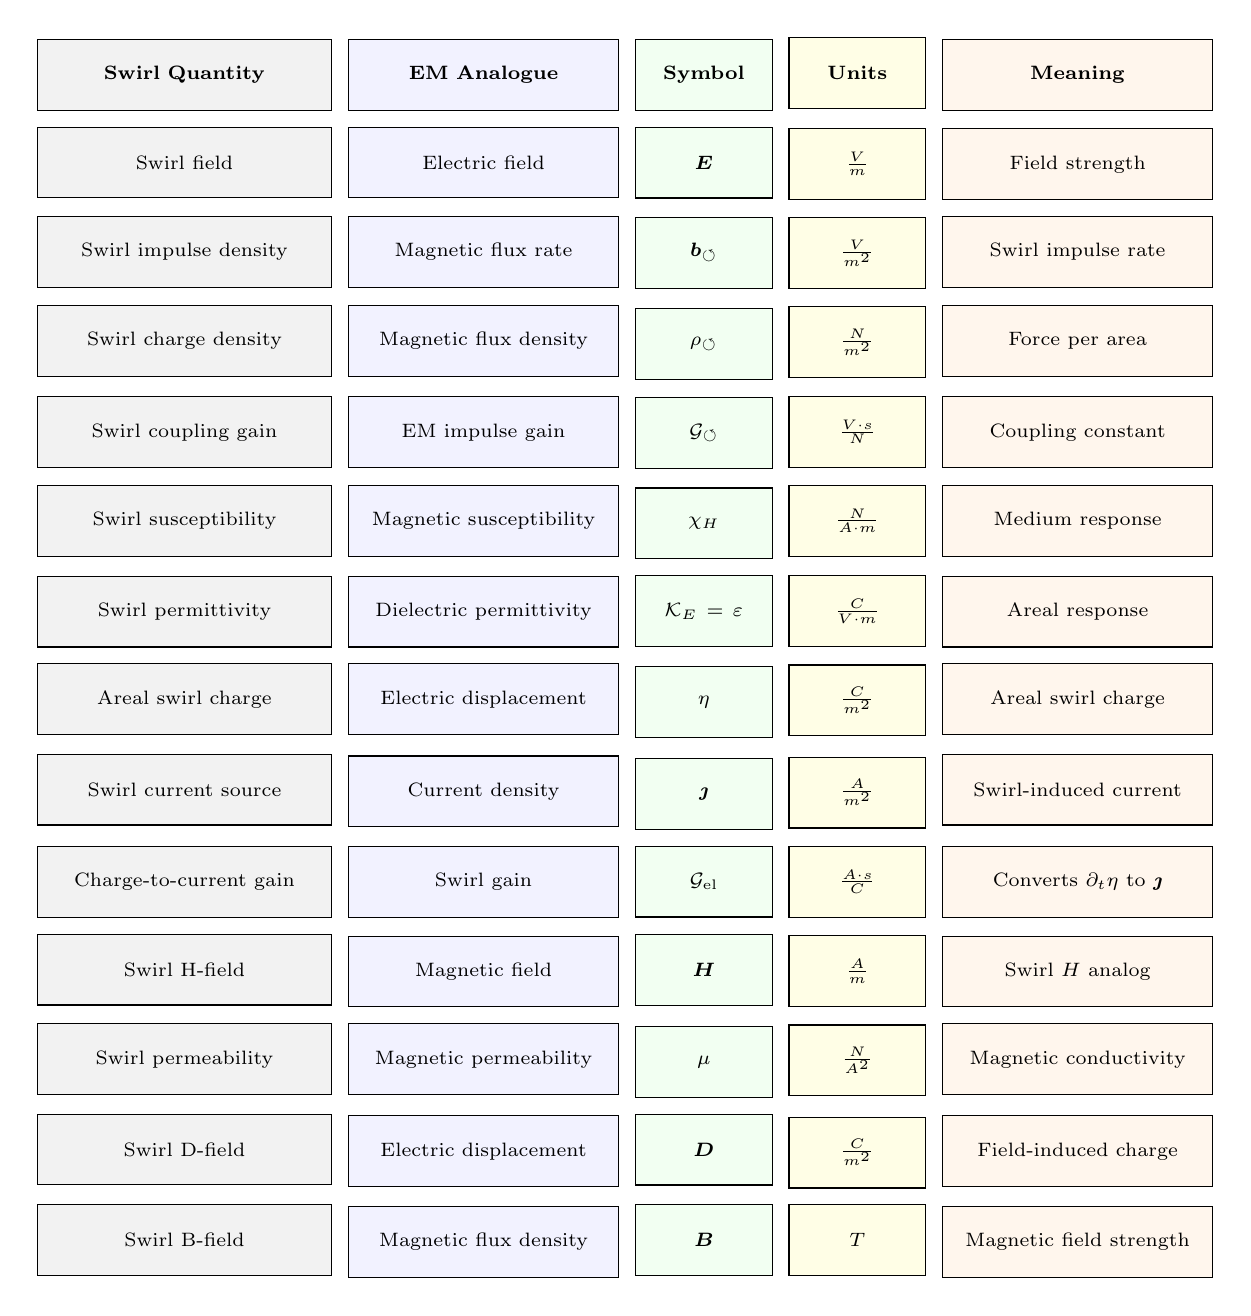
\begin{tikzpicture}
    \tikzset{
        tablecell/.style={
            draw, align=center, font=\scriptsize,
            text height=1.9ex, text depth=.6ex,
            inner sep=2pt, minimum height=0.9cm
        }
    }
    \matrix[matrix of nodes,
        nodes={draw, align=center, font=\scriptsize, text width=3.2cm, minimum height=0.9cm},
        column sep=0.2cm, row sep=0.2cm,
        column 1/.style={nodes={text width=3.5cm, fill=gray!10}},
        column 2/.style={nodes={fill=blue!5}},
        column 3/.style={nodes={text width=1.5cm, fill=green!5}},
        column 4/.style={nodes={text width=1.5cm, fill=yellow!10}},
        column 5/.style={nodes={fill=orange!7}}
    ] (m) {
        \textbf{Swirl Quantity} & \textbf{EM Analogue} & \textbf{Symbol} & \textbf{Units} & \textbf{Meaning} \\
        Swirl field & Electric field & $\EE$ & $\tfrac{V}{m}$ & Field strength \\
        Swirl impulse density & Magnetic flux rate & $\vect{b}_{\circlearrowleft}$ & $\tfrac{V}{m^2}$ & Swirl impulse rate \\
        Swirl charge density & Magnetic flux density & $\rho_{\circlearrowleft}$ & $\tfrac{N}{m^2}$ & Force per area \\
        Swirl coupling gain & EM impulse gain & $\mathcal{G}_{\circlearrowleft}$ & $\tfrac{V\cdot s}{N}$ & Coupling constant \\
        Swirl susceptibility & Magnetic susceptibility & $\chi_H$ & $\tfrac{N}{A \cdot m}$ & Medium response \\
        Swirl permittivity & Dielectric permittivity & $\mathcal{K}_E = \varepsilon$ & $\tfrac{C}{V \cdot m}$ & Areal response \\
        Areal swirl charge & Electric displacement & $\eta$ & $\tfrac{C}{m^2}$ & Areal swirl charge \\
        Swirl current source & Current density & $\jj$ & $\tfrac{A}{m^2}$ & Swirl-induced current \\
        Charge-to-current gain & Swirl gain & $\mathcal{G}_{\mathrm{el}}$ & $\tfrac{A \cdot s}{C}$ & Converts $\partial_t \eta$ to $\jj$ \\
        Swirl H-field & Magnetic field & $\HH$ & $\tfrac{A}{m}$ & Swirl $H$ analog \\
        Swirl permeability & Magnetic permeability & $\mu$ & $\tfrac{N}{A^2}$ & Magnetic conductivity \\
        Swirl D-field & Electric displacement & $\DD$ & $\tfrac{C}{m^2}$ & Field-induced charge \\
        Swirl B-field & Magnetic flux density & $\BB$ & $T$ & Magnetic field strength \\
    };
    \end{tikzpicture}
    \caption{Canonical Swirl–Electromagnetic Unit Bridge Table.}
    \label{fig:swirl_em_units}
    \end{figure}
    }

\end{document}
